\documentclass[conference]{IEEEtran}
\usepackage{booktabs} % For formal tables
\newenvironment{itemize*}{\begin{itemize}}{\end{itemize}}
\usepackage[utf8x]{inputenc}
\usepackage{subfigure}
\usepackage{balance}
\usepackage{comment}
\usepackage{amsmath}
\usepackage{xspace}
\usepackage{caption}
\usepackage{siunitx}
\usepackage{booktabs}
% Some Computer Society conferences also require the compsoc mode option,
% but others use the standard conference format.
%
% If IEEEtran.cls has not been installed into the LaTeX system files,
% manually specify the path to it like:
% \documentclass[conference]{../sty/IEEEtran}





% Some very useful LaTeX packages include:
% (uncomment the ones you want to load)


% *** MISC UTILITY PACKAGES ***
%
%\usepackage{ifpdf}
% Heiko Oberdiek's ifpdf.sty is very useful if you need conditional
% compilation based on whether the output is pdf or dvi.
% usage:
% \ifpdf
%   % pdf code
% \else
%   % dvi code
% \fi
% The latest version of ifpdf.sty can be obtained from:
% http://www.ctan.org/pkg/ifpdf
% Also, note that IEEEtran.cls V1.7 and later provides a builtin
% \ifCLASSINFOpdf conditional that works the same way.
% When switching from latex to pdflatex and vice-versa, the compiler may
% have to be run twice to clear warning/error messages.






% *** CITATION PACKAGES ***
%
\usepackage{cite}
% cite.sty was written by Donald Arseneau
% V1.6 and later of IEEEtran pre-defines the format of the cite.sty package
% \cite{} output to follow that of the IEEE. Loading the cite package will
% result in citation numbers being automatically sorted and properly
% "compressed/ranged". e.g., [1], [9], [2], [7], [5], [6] without using
% cite.sty will become [1], [2], [5]--[7], [9] using cite.sty. cite.sty's
% \cite will automatically add leading space, if needed. Use cite.sty's
% noadjust option (cite.sty V3.8 and later) if you want to turn this off
% such as if a citation ever needs to be enclosed in parenthesis.
% cite.sty is already installed on most LaTeX systems. Be sure and use
% version 5.0 (2009-03-20) and later if using hyperref.sty.
% The latest version can be obtained at:
% http://www.ctan.org/pkg/cite
% The documentation is contained in the cite.sty file itself.






% *** GRAPHICS RELATED PACKAGES ***
%
\ifCLASSINFOpdf
 \usepackage[pdftex]{graphicx}
  % declare the path(s) where your graphic files are
  % \graphicspath{{../pdf/}{../jpeg/}}
  % and their extensions so you won't have to specify these with
  % every instance of \includegraphics
 \DeclareGraphicsExtensions{.pdf,.jpeg,.png}
\else
  % or other class option (dvipsone, dvipdf, if not using dvips). graphicx
  % will default to the driver specified in the system graphics.cfg if no
  % driver is specified.
 \usepackage[dvips]{graphicx}
  % declare the path(s) where your graphic files are
  % \graphicspath{{../eps/}}
  % and their extensions so you won't have to specify these with
  % every instance of \includegraphics
 \DeclareGraphicsExtensions{.eps}
\fi
% graphicx was written by David Carlisle and Sebastian Rahtz. It is
% required if you want graphics, photos, etc. graphicx.sty is already
% installed on most LaTeX systems. The latest version and documentation
% can be obtained at: 
% http://www.ctan.org/pkg/graphicx
% Another good source of documentation is "Using Imported Graphics in
% LaTeX2e" by Keith Reckdahl which can be found at:
% http://www.ctan.org/pkg/epslatex
%
% latex, and pdflatex in dvi mode, support graphics in encapsulated
% postscript (.eps) format. pdflatex in pdf mode supports graphics
% in .pdf, .jpeg, .png and .mps (metapost) formats. Users should ensure
% that all non-photo figures use a vector format (.eps, .pdf, .mps) and
% not a bitmapped formats (.jpeg, .png). The IEEE frowns on bitmapped formats
% which can result in "jaggedy"/blurry rendering of lines and letters as
% well as large increases in file sizes.
%
% You can find documentation about the pdfTeX application at:
% http://www.tug.org/applications/pdftex





% *** MATH PACKAGES ***
%
\usepackage{amsmath}
\usepackage{amssymb}
% A popular package from the American Mathematical Society that provides
% many useful and powerful commands for dealing with mathematics.
%
% Note that the amsmath package sets \interdisplaylinepenalty to 10000
% thus preventing page breaks from occurring within multiline equations. Use:
%\interdisplaylinepenalty=2500
% after loading amsmath to restore such page breaks as IEEEtran.cls normally
% does. amsmath.sty is already installed on most LaTeX systems. The latest
% version and documentation can be obtained at:
% http://www.ctan.org/pkg/amsmath





% *** SPECIALIZED LIST PACKAGES ***
%
%\usepackage{algorithmic}
% algorithmic.sty was written by Peter Williams and Rogerio Brito.
% This package provides an algorithmic environment fo describing algorithms.
% You can use the algorithmic environment in-text or within a figure
% environment to provide for a floating algorithm. Do NOT use the algorithm
% floating environment provided by algorithm.sty (by the same authors) or
% algorithm2e.sty (by Christophe Fiorio) as the IEEE does not use dedicated
% algorithm float types and packages that provide these will not provide
% correct IEEE style captions. The latest version and documentation of
% algorithmic.sty can be obtained at:
% http://www.ctan.org/pkg/algorithms
% Also of interest may be the (relatively newer and more customizable)
% algorithmicx.sty package by Szasz Janos:
% http://www.ctan.org/pkg/algorithmicx




% *** ALIGNMENT PACKAGES ***
%
%\usepackage{array}
% Frank Mittelbach's and David Carlisle's array.sty patches and improves
% the standard LaTeX2e array and tabular environments to provide better
% appearance and additional user controls. As the default LaTeX2e table
% generation code is lacking to the point of almost being broken with
% respect to the quality of the end results, all users are strongly
% advised to use an enhanced (at the very least that provided by array.sty)
% set of table tools. array.sty is already installed on most systems. The
% latest version and documentation can be obtained at:
% http://www.ctan.org/pkg/array


% IEEEtran contains the IEEEeqnarray family of commands that can be used to
% generate multiline equations as well as matrices, tables, etc., of high
% quality.




% *** SUBFIGURE PACKAGES ***
%\ifCLASSOPTIONcompsoc
%  \usepackage[caption=false,font=normalsize,labelfont=sf,textfont=sf]{subfig}
%\else
%  \usepackage[caption=false,font=footnotesize]{subfig}
%\fi
% subfig.sty, written by Steven Douglas Cochran, is the modern replacement
% for subfigure.sty, the latter of which is no longer maintained and is
% incompatible with some LaTeX packages including fixltx2e. However,
% subfig.sty requires and automatically loads Axel Sommerfeldt's caption.sty
% which will override IEEEtran.cls' handling of captions and this will result
% in non-IEEE style figure/table captions. To prevent this problem, be sure
% and invoke subfig.sty's "caption=false" package option (available since
% subfig.sty version 1.3, 2005/06/28) as this is will preserve IEEEtran.cls
% handling of captions.
% Note that the Computer Society format requires a larger sans serif font
% than the serif footnote size font used in traditional IEEE formatting
% and thus the need to invoke different subfig.sty package options depending
% on whether compsoc mode has been enabled.
%
% The latest version and documentation of subfig.sty can be obtained at:
% http://www.ctan.org/pkg/subfig




% *** FLOAT PACKAGES ***
%
%\usepackage{fixltx2e}
% fixltx2e, the successor to the earlier fix2col.sty, was written by
% Frank Mittelbach and David Carlisle. This package corrects a few problems
% in the LaTeX2e kernel, the most notable of which is that in current
% LaTeX2e releases, the ordering of single and double column floats is not
% guaranteed to be preserved. Thus, an unpatched LaTeX2e can allow a
% single column figure to be placed prior to an earlier double column
% figure.
% Be aware that LaTeX2e kernels dated 2015 and later have fixltx2e.sty's
% corrections already built into the system in which case a warning will
% be issued if an attempt is made to load fixltx2e.sty as it is no longer
% needed.
% The latest version and documentation can be found at:
% http://www.ctan.org/pkg/fixltx2e


%\usepackage{stfloats}
% stfloats.sty was written by Sigitas Tolusis. This package gives LaTeX2e
% the ability to do double column floats at the bottom of the page as well
% as the top. (e.g., "\begin{figure*}[!b]" is not normally possible in
% LaTeX2e). It also provides a command:
%\fnbelowfloat
% to enable the placement of footnotes below bottom floats (the standard
% LaTeX2e kernel puts them above bottom floats). This is an invasive package
% which rewrites many portions of the LaTeX2e float routines. It may not work
% with other packages that modify the LaTeX2e float routines. The latest
% version and documentation can be obtained at:
% http://www.ctan.org/pkg/stfloats
% Do not use the stfloats baselinefloat ability as the IEEE does not allow
% \baselineskip to stretch. Authors submitting work to the IEEE should note
% that the IEEE rarely uses double column equations and that authors should try
% to avoid such use. Do not be tempted to use the cuted.sty or midfloat.sty
% packages (also by Sigitas Tolusis) as the IEEE does not format its papers in
% such ways.
% Do not attempt to use stfloats with fixltx2e as they are incompatible.
% Instead, use Morten Hogholm'a dblfloatfix which combines the features
% of both fixltx2e and stfloats:
%
% dblfloatfix}
% The latest version can be found at:
% http://www.ctan.org/pkg/dblfloatfix




% *** PDF, URL AND HYPERLINK PACKAGES ***
%
\usepackage{url}
% url.sty was written by Donald Arseneau. It provides better support for
% handling and breaking URLs. url.sty is already installed on most LaTeX
% systems. The latest version and documentation can be obtained at:
% http://www.ctan.org/pkg/url
% Basically, \url{my_url_here}.

% For special characters like ä,ö,...
\usepackage[utf8x]{inputenc}


% *** Do not adjust lengths that control margins, column widths, etc. ***
% *** Do not use packages that alter fonts (such as pslatex).         ***
% There should be no need to do such things with IEEEtran.cls V1.6 and later.
% (Unless specifically asked to do so by the journal or conference you plan
% to submit to, of course. )


% correct bad hyphenation here
\hyphenation{op-tical net-works semi-conduc-tor}

\newcommand{\cp}[1]{\footnote{{\bf Carlos: #1}}}
\newcommand{\fakeparagraph}[1]{\vspace{.5mm}\noindent\textbf{#1.}}
\newcommand{\fakepar}[1]{\fakeparagraph{#1}}

\begin{document}
%
% paper title
% Titles are generally capitalized except for words such as a, an, and, as,
% at, but, by, for, in, nor, of, on, or, the, to and up, which are usually
% not capitalized unless they are the first or last word of the title.
% Linebreaks \\ can be used within to get better formatting as desired.
% Do not put math or special symbols in the title.
\title{Enabling Ambient Backscatter \\Using a Low-Cost Software Defined Radio}


% author names and affiliations
% use a multiple column layout for up to three different
% affiliations
\author{\IEEEauthorblockN{Maximilian Stiefel}
\IEEEauthorblockA{Master Programme Embdedded Systems\\
Uppsala University\\
maximilian.stiefel.8233@student.uu.se}
\and
\IEEEauthorblockN{Elmar van Rijnswou}
\IEEEauthorblockA{Master Programme Embdedded Systems\\
Uppsala University\\
elmar.vanrijnswou.9818@student.uu.se}
\and
\IEEEauthorblockN{Carlos Pérez-Penichet}
\IEEEauthorblockA{Uppsala University\\
carlos.penichet@it.uu.se}
\and
\IEEEauthorblockN{Ambuj Varshney}
\IEEEauthorblockA{Uppsala University\\
ambuj.varshney@it.uu.se}
\and
\IEEEauthorblockN{Christian Rohner}
\IEEEauthorblockA{Uppsala University\\
christian.rohner@it.uu.se}
\and
\IEEEauthorblockN{Thiemo Voigt}
\IEEEauthorblockA{Uppsala University\\
and SICS Swedish ICT\\
thiemo@sics.se}}

% conference papers do not typically use \thanks and this command
% is locked out in conference mode. If really needed, such as for
% the acknowledgment of grants, issue a \IEEEoverridecommandlockouts
% after \documentclass

% for over three affiliations, or if they all won't fit within the width
% of the page, use this alternative format:
% 
%\author{\IEEEauthorblockN{Michael Shell\IEEEauthorrefmark{1},
%Homer Simpson\IEEEauthorrefmark{2},
%James Kirk\IEEEauthorrefmark{3}, 
%Montgomery Scott\IEEEauthorrefmark{3} and
%Eldon Tyrell\IEEEauthorrefmark{4}}
%\IEEEauthorblockA{\IEEEauthorrefmark{1}School of Electrical and Computer Engineering\\
%Georgia Institute of Technology,
%Atlanta, Georgia 30332--0250\\ Email: see http://www.michaelshell.org/contact.html}
%\IEEEauthorblockA{\IEEEauthorrefmark{2}Twentieth Century Fox, Springfield, USA\\
%Email: homer@thesimpsons.com}
%\IEEEauthorblockA{\IEEEauthorrefmark{3}Starfleet Academy, San Francisco, California 96678-2391\\
%Telephone: (800) 555--1212, Fax: (888) 555--1212}
%\IEEEauthorblockA{\IEEEauthorrefmark{4}Tyrell Inc., 123 Replicant Street, Los Angeles, California 90210--4321}}




% use for special paper notices
%\IEEEspecialpapernotice{(Invited Paper)}




% make the title area
\maketitle

% As a general rule, do not put math, special symbols or citations
% in the abstract
\begin{abstract}
Backscatter communication is attractive for energy-constrained devices
				due to its very low power requirements. Ambient backscatter
				takes this point to the limit by leveraging existing radio
				frequency signals for the purpose of communication, without the
				need for generating an energy-expensive carrier signal. In this
				paper we investigate the use of television broadcast signals as
				a carrier for backscatter communication. As opposed to the
				state-of-the-art, restricted to operations under conditions of
				high signal strength, we demonstrate a low-cost software defined
				radio receiver that operates even in conditions when ambient
				signals are weak. We build the system using a low-cost
				off-the-shelf microcontroller and an RTLSDR software-defined
				radio receiver. We also conduct a survey of the signal strength
				of TV broadcast in a mid-sized Swedish city and observe that our
				system can operate in most parts of the city.
\end{abstract}

% no keywords




% For peer review papers, you can put extra information on the cover
% page as needed:
% \ifCLASSOPTIONpeerreview
% \begin{center} \bfseries EDICS Category: 3-BBND \end{center}
% \fi
%
% For peerreview papers, this IEEEtran command inserts a page break and
% creates the second title. It will be ignored for other modes.
\IEEEpeerreviewmaketitle



\section{Introduction}
% no \IEEEPARstart
% You must have at least 2 lines in the paragraph with the drop letter
% (should never be an issue)

Backscatter communication enables wireless transmissions
at energy consumption which is several orders of magnitude
lower than traditional radios. Backscatter achieves ultra-low
power wireless transmissions by reflecting or absorbing ambient
wireless signals, which as an operation consumes only 
\SI{}{\micro\watt}s of power consumption~\cite{liu_ambient_2013}. 
As a consequence backscatter
communication is emerging as the mechanism of choice to network
devices operating on harvested energy.  
Over the past few years there has been significant progress
to make backscatter a viable mechanism to network Internet of
Things~(IoT) devices. Traditional backscatter systems, like RFID readers, required a
dedicated device to generate the necessary carrier signal
reflected by the tags. On the other hand, state-of-the art systems 
does away the need for a dedicated device to generate carrier signals. 
Recent backscatter systems leverage already deployed infrastructure of
devices to generate carrier signal~\cite{varshney2016lorea,iyer2016inter}, or ambient WiFi~\cite{hitchhike,kellogg2015wi} or TV
signals~\cite{liu_ambient_2013,parks_turbocharging_2014}.

Recent backscatter systems demonstrate ability to leverage
existing signals like TV signals as a both source of carrier and energy. For
example, Liu et al. present a proof-of-concept system that reflects
ambient TV signals and enables tag-to-tag communication up to almost a
meter. Parks et al. further improve the communication range to several
meters by using analog coding~\cite{parks_turbocharging_2014}. While
these systems can enable many applications, these systems are severely restricted
to operate in the vicinity of television towers where ambient signal
are sufficiently strong~(approx
\SI{-30}{dBm}). This is primarily due to poor sensitivity levels of receivers
employed on these devices, which together with weak backscatter reflections 
severely limits the operating range from the tower.
On the other hand, TV signals are known to vary greatly in
strength~\cite{wang_fm_2017} both over space, and in time,  which further aggravates the
problem of limited range of ambient backscatter systems.

On the other hand, Software Defined Radios~(SDRs) are powerful devices, and also
have significant processing abilities. These devices offer high
sensitivity levels, as compared to the receivers employed on typical 
ambient backscatter tags. Thus, SDRs might help to
significantly improve the communication range, and also coverage 
area to receive ambient backscatter transmissions. 

In this paper we explore the following questions: Can we leverage an
SDR-based receiver to receive ambient backscatter transmissions ?, and, Does the  
relatively high sensitivity of SDR receivers improve
range and coverage of ambient backscatter systems? A positive answer to the above question would provide a
flexible and low-cost experimentation platform to the wider research community to explore ambient backscatter
systems.

\fakepar{Contributions}  In this paper, we make the following novel contributions:

\begin{itemize}
		

				\item We design the first system which leverages a  low-cost 
					  SDR to receive ambient-backscatter transmissions. 
				\item  Using the system designed, we demonstrate ambient backscatter using TV signals
					   to be feasible in wide parts of a city. The range represents a significant improvement
					   over the state-of-the-art.
				
\end{itemize}



% An example of a floating figure using the graphicx package.
% Note that \label must occur AFTER (or within) \caption.
% For figures, \caption should occur after the \includegraphics.
% Note that IEEEtran v1.7 and later has special internal code that
% is designed to preserve the operation of \label within \caption
% even when the captionsoff option is in effect. However, because
% of issues like this, it may be the safest practice to put all your
% \label just after \caption rather than within \caption{}.
%
% Reminder: the "draftcls" or "draftclsnofoot", not "draft", class
% option should be used if it is desired that the figures are to be
% displayed while in draft mode.
%
%\begin{figure}[!t]
%\centering
%\includegraphics[width=2.5in]{myfigure}
% where an .eps filename suffix will be assumed under latex, 
% and a .pdf suffix will be assumed for pdflatex; or what has been declared
% via \DeclareGraphicsExtensions.
%\caption{Simulation results for the network.}
%\label{fig_sim}
%\end{figure}

% Note that the IEEE typically puts floats only at the top, even when this
% results in a large percentage of a column being occupied by floats.


% An example of a double column floating figure using two subfigures.
% (The subfig.sty package must be loaded for this to work.)
% The subfigure \label commands are set within each subfloat command,
% and the \label for the overall figure must come after \caption.
% \hfil is used as a separator to get equal spacing.
% Watch out that the combined width of all the subfigures on a 
% line do not exceed the text width or a line break will occur.
%
%\begin{figure*}[!t]
%\centering
%\subfloat[Case I]{\includegraphics[width=2.5in]{box}%
%\label{fig_first_case}}
%\hfil
%\subfloat[Case II]{\includegraphics[width=2.5in]{box}%
%\label{fig_second_case}}
%\caption{Simulation results for the network.}
%\label{fig_sim}
%\end{figure*}
%
% Note that often IEEE papers with subfigures do not employ subfigure
% captions (using the optional argument to \subfloat[]), but instead will
% reference/describe all of them (a), (b), etc., within the main caption.
% Be aware that for subfig.sty to generate the (a), (b), etc., subfigure
% labels, the optional argument to \subfloat must be present. If a
% subcaption is not desired, just leave its contents blank,
% e.g., \subfloat[].


% An example of a floating table. Note that, for IEEE style tables, the
% \caption command should come BEFORE the table and, given that table
% captions serve much like titles, are usually capitalized except for words
% such as a, an, and, as, at, but, by, for, in, nor, of, on, or, the, to
% and up, which are usually not capitalized unless they are the first or
% last word of the caption. Table text will default to \footnotesize as
% the IEEE normally uses this smaller font for tables.
% The \label must come after \caption as always.
%
%\begin{table}[!t]
%% increase table row spacing, adjust to taste
%\renewcommand{\arraystretch}{1.3}
% if using array.sty, it might be a good idea to tweak the value of
% \extrarowheight as needed to properly center the text within the cells
%\caption{An Example of a Table}
%\label{table_example}
%\centering
%% Some packages, such as MDW tools, offer better commands for making tables
%% than the plain LaTeX2e tabular which is used here.
%\begin{tabular}{|c||c|}
%\hline
%One & Two\\
%\hline
%Three & Four\\
%\hline
%\end{tabular}
%\end{table}


% Note that the IEEE does not put floats in the very first column
% - or typically anywhere on the first page for that matter. Also,
% in-text middle ("here") positioning is typically not used, but it
% is allowed and encouraged for Computer Society conferences (but
% not Computer Society journals). Most IEEE journals/conferences use
% top floats exclusively. 
% Note that, LaTeX2e, unlike IEEE journals/conferences, places
% footnotes above bottom floats. This can be corrected via the
% \fnbelowfloat command of the stfloats package.

\section{Background}

In this background section we introduce the necessary knowledge about sofware defined radios and the used hardware, the \textit{RTL-SDR}.  

\subsection{Software Defined Radio}
Traditionally basic radio components like mixers or filters have been realized
in hardware. Nowadays as soon as one works in the baseband frequency the
computational resources of a personal computer are sufficient to realize these
components with signal processing done in software. \cp{We need to expand on
this introduction to SDR, assuming we need it and not just assume everyone
knows what that is.}

\subsection{RTL2832U}
\label{sub:rtl2832}
 \begin{figure}[h]
 \centering
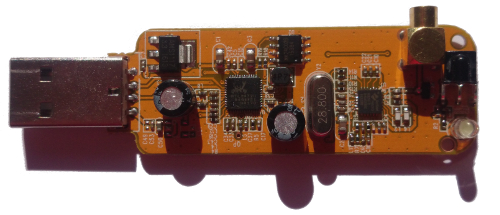
\includegraphics[width=0.5\columnwidth]{./fig/rtlsdr.jpg}
\caption{\textit{RTL-SDR} hardware with the DVB-T I/Q demodulator
\textit{Raeltek RTL2832U} (left IC) and the tuner with integrated LNA
\textit{Rafael Micro R820T/2} (right IC).}
 \label{fig:receiver_arch}
\end{figure}
The \textit{Realtek RTL2832U} is a terrestrial digital video broadcast
(DVB-T) demodulator IC, which is the main part of a wide range of
USB-based DVB-T receiver dongles. One prominent feature of this chip is
that it allows to retrieve the raw I/Q samples via USB. This is
originally intended for the chip to work as a simple DAB/FM software
receiver. Ham radio enthusiasts have combined their efforts to create a
software driver (the \textit{librtlsdr}, cf. \cite{steve-m_librtlsdr})
that allows DVB-T dongles based on the \textit{RTL2832} to be converted
into low-cost wideband SDR receivers. The cost of traditional SDRs has
been in the range of a few hundred to thousands of USD. Albeit much less
powerful than a typical SDR, a \textit{RTL2832U}-based DVB-T receiver
can be bought with antenna for less than 10 USD.  A RTL-SDR does not
only consist of the \textit{RTL2832U}, but also a tuner. The tuner is an
essential component, as it allows the user to select the received
frequency and outputs that signal at an intermediate frequency (IF). The
IF can then be fed into the demodulator for digitalization. In the case
of the used hardware this tuner is a \textit{Rafael Micro R820T/2} which
offers a tuning range from 42 to 1002 MHz~\cite{rafael_r820t_2011}. It
subsumes a low-noise amplifier (LNA) and filters. It presents a low
noise figure of 3.5 dB and features 65 dBc of image rejection. Figure
\ref{fig:receiver_arch}, shows a photograph of the RTL-SDR used in our
work. 

\subsection{Quadrature Demodulation}

The received signal can be interpreted as
\begin{equation}
	s_{\text{IF}}(t)=I(t) \cdot cos(\omega_{0}t) + Q(t) \cdot sin(\omega_{0}t)
\end{equation}     
This is multiplied with a cosine (and a sine as well) from a local oscillator.
\begin{multline}
        s_{\text{IF}}(t) \cdot s_\text{L}(t) = I(t) \cdot cos(\omega_{0}t) \cdot cos(\omega_{0}t)\\+ Q(t) \cdot sin(\omega_{0}t) \cdot cos(\omega_{0}t)
\end{multline}
With \ensuremath{2\,cos(a)cos(b)=cos(a-b)+cos(a+b)} and \ensuremath{2\,sin(a)cos(b)=sin(a+b)+sin(a-b)} follows
\begin{multline}
        2 \cdot s_{\text{IF}}(t) \cdot s_L(t) = I(t) \cdot \bigl[1+cos(2\omega_{0}t)\bigr]\\+ Q(t) \cdot \bigl[sin(2\omega_0t)+sin(0)\bigr].
\end{multline}
One can see, that the interesting in-phase part (I) in this case is
represented by a DC value after mixing. With a low-pass filter this DC
value can be separated from the undesired rest. An analogous procedure
is done with the quadrature part (Q) when mixing with a sine.

\section{Design}

\subsection{Transmitter}
\begin{figure}[h]
\centering
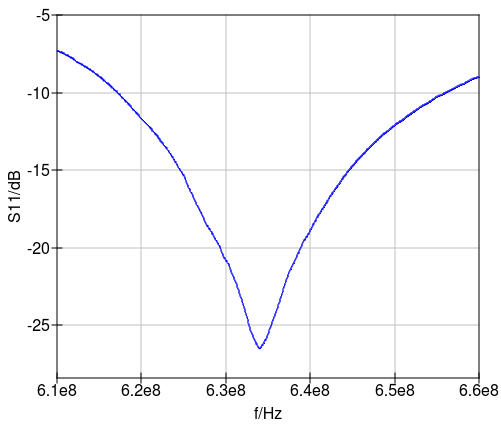
\includegraphics[width=0.6\columnwidth]{./fig/s11v2}
\caption{Input reflection coefficient \ensuremath{\Gamma_{in}} also known as \ensuremath{S_{\text{11}}} of the self-made backscattering ground-plane antenna.}
\label{fig:s11}
\end{figure}
 
Our backscattering antenna is optimized for usage with the television signal,
which has its center frequency at 626 MHz. It is a ground plane antenna, which
has been built up on a large unetched PCB plate. A hole in the middle of the
PCB serves for connecting a wire to a 50 \ensuremath{\Omega} micro strip
transmission line. The wire, which acts as a vertical antenna element is
soldered to the transmission line. The microstrip transmission line design
equations given in \cite{pozar_microwave_2011} are implemented in various
programs e.g.  KiCAD, which has been used for designing them. An open-stub,
attached directly at the juncture where the vertical antenna element is
attached to the transmission line, is used for fine tuning of the input
impedance (cf. chapter 5 in \cite{pozar_microwave_2011}).  Accepting -15 dB as
sufficient value for \ensuremath{S_{11}}, one can say, that the antenna works
within a range from 626 MHz to 645 MHz. With our narrowband antenna the
undesired backscattering of out-of-band signals is reduced. With our approach
we were able to achieve an input impedance at 634 MHz of
\ensuremath{Z_{in}=(52.2 + j 4.3) \Omega}. At 626 MHz
\ensuremath{S_{\text{11}}} is still approximately -17 dB.

Besides the antenna, the transmitter consists of an \textit{MSP430} MCU,
that sends data to the receiver. This transmitter controls an RF switch
through an I/O pin. The switch can alternate the impedance connected to
the antenna between matched (50 \ensuremath{\Omega}) and open. The
software now steers this switch with a two 2 MHz rectangular timer
signal to transmit a data 1 or it just leaves the antenna open to
transmit a data 0. Therefore the result is a frequency shift of the
television signal by 2 MHz for a 1 and no shift for a 0. This can be
easily understood thinking about a simple cosine, which is shifted by
another cosine: \ensuremath{2\,cos(a)cos(b)=cos(a-b)+cos(a+b)}. Of
course this example is simplified compared to the actual situation as
the actual signal, which is used for shifting contains more than one
frequency as well as the TV signal, which is shifted. Hence a classical
binary amplitude shift keying is the implemented modulation technique.   
 
\subsection{Receiver}
\begin{figure}[h]
\centering
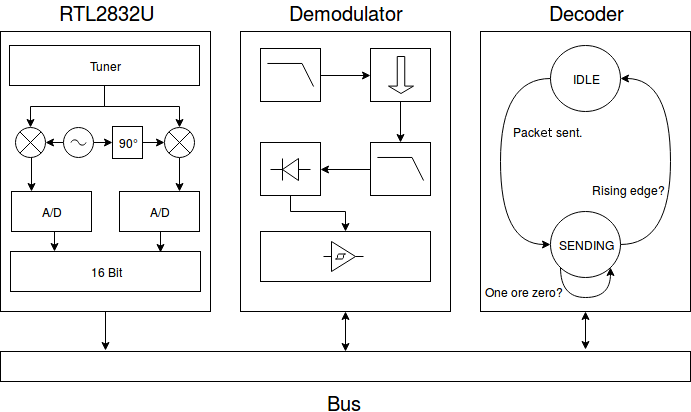
\includegraphics[width=\columnwidth]{./fig/receiver_arch}
\caption{Receiver architecture from a system point of view. Signal flow is from left to right.}
\label{fig:receiver_arch}
\end{figure}
We provide our C++ receiver code publicly available under
\url{https://github.com/s3xm3x/backscatterBASKReceiver}. A highly sophisticated
bus system has been developed to exchange data between the different components
of the system. The signal flow in figure \ref{fig:receiver_arch} is from the
left to the right.  \textit{Librtlsdr} (cf. \cite{steve-m_librtlsdr}), which is
based on \textit{libusb}, is used to transfer the data from the TV stick into
our program. As described in section~\ref{sub:rtl2832}, the RTL2832 mixes down
the high frequency to a intermediate frequency (both values are software
adjustable). The sampled data is available as two 8-bit values (real and
imaginary). With this two values, the phase and absolute value of the data can
be determined for every sample. Every sample can be intepreted as:
\begin{equation}
	I+j\,Q = abs(I,Q) \cdot e^{j \times ang(I,Q)} 
\end{equation} 
 
So the first block, which is entitled RTL2832U, provides the interface to the
TV dongle. This block controls the frequency \ensuremath{f_{tuned}}, where the
receiver is listening, besides other interesting parameters e.g. the analog
gain.

The demodulator block is responsible for converting the sampled signals into
ones and zeroes. Therefore the real and imaginary values first have to be
deinterleaved out of the sample message. These 8 bit integers are converted
into floats, whereas 127.5 equals 0. After that the values have to be
downsampled. Usually we were sampling with 250 kHz. This is still much more
than we need assuming an Additive White Gaussian Noise (AWGN) channel with a
\ensuremath{S/N = 10\,dB} (cf.  equation \ref{eq:awgn}).  So we decided to
reduce the sampling frequency to 25 kHz.
 
\begin{equation}
	\label{eq:awgn}
	C=B \cdot log_2(1+\frac{S}{N})= 25\,kHz \cdot log_2(11) \approx 86.5\,kbit/s
\end{equation}     
To do this it is important to use an anti-aliasing filter, as the Shannon-Nyquist theorem has to be satisfied: 
\begin{equation}
	\label{eq:nyquist}
	f_{samp} \geq 2 \cdot f_{a}
\end{equation}
\ensuremath{f_{a}} is the highest frequency in the signal. 
 A FIR filter
naively implemented with floats has been used to achieve this.  After
downsampling another filter is used to suppress noise.  The last demodulation
step is to rectify the signal (cf. equation \ref{eq:rectify}) and decide with a
software-defined Schmitt trigger whether a sample is a 1 or a 0.  
\begin{equation}
	\label{eq:rectify}
	abs(I,Q) = \sqrt{I^2 +  Q^2}
\end{equation} 
A registered listener receives the processed samples, which are broadcasted by
the demodulator. This registered listener is the decoder. After the decoder
received the samples it decides when a frame is sent or when the channel is
idle.  The decoder also includes a function to correlate the received bitstream
with an expected pattern. Hence it is able to determine the bit error ratio
(BER). Furthermore the code we have written so far subsumes different
simulators for e.g. playing back recoreded data. Another handy utility, which
has been written in Octave, is a tool (an oscilloscope) to look at the data,
which is written into files by the demodulator (cf. figure \ref{fig:transmission}).
\begin{figure}[h]
 
\centering
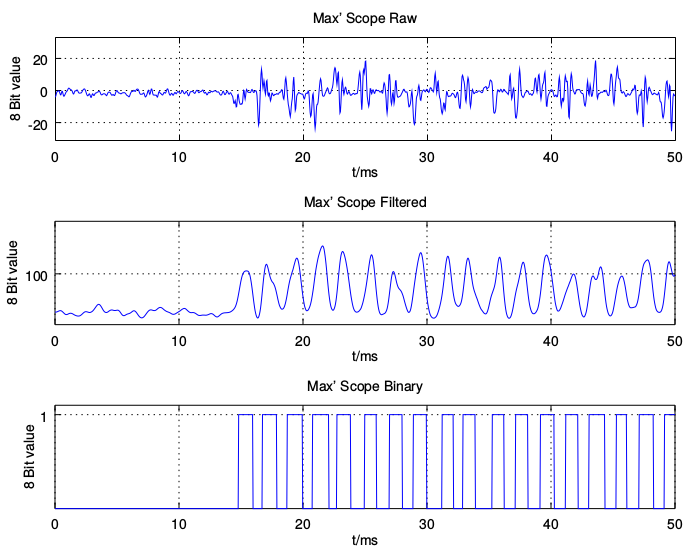
\includegraphics[width=\columnwidth]{./fig/transmission}
\caption{Start of a transmission of 101010.. with 1 kbit/s with idle state before. Data from the Octave oscilloscope. Amplitude is quite low with an average of 12 \% of the maximum, which is 127.5. This is due to a low signal strength. Sampling frequency is 25 kHz.}
\label{fig:transmission}
\end{figure}

\section{Evaluation}
In this section we present our evaluation results. The \textit{RTL-SDR},
combined with intelligent signal processing in \textit{Octave}, are the
main tools we have employed for measurements. 

\subsection{Signal Strength Variation in Space}
\begin{figure}[h]
	\centering
	\begin{minipage}{0.49\columnwidth}
	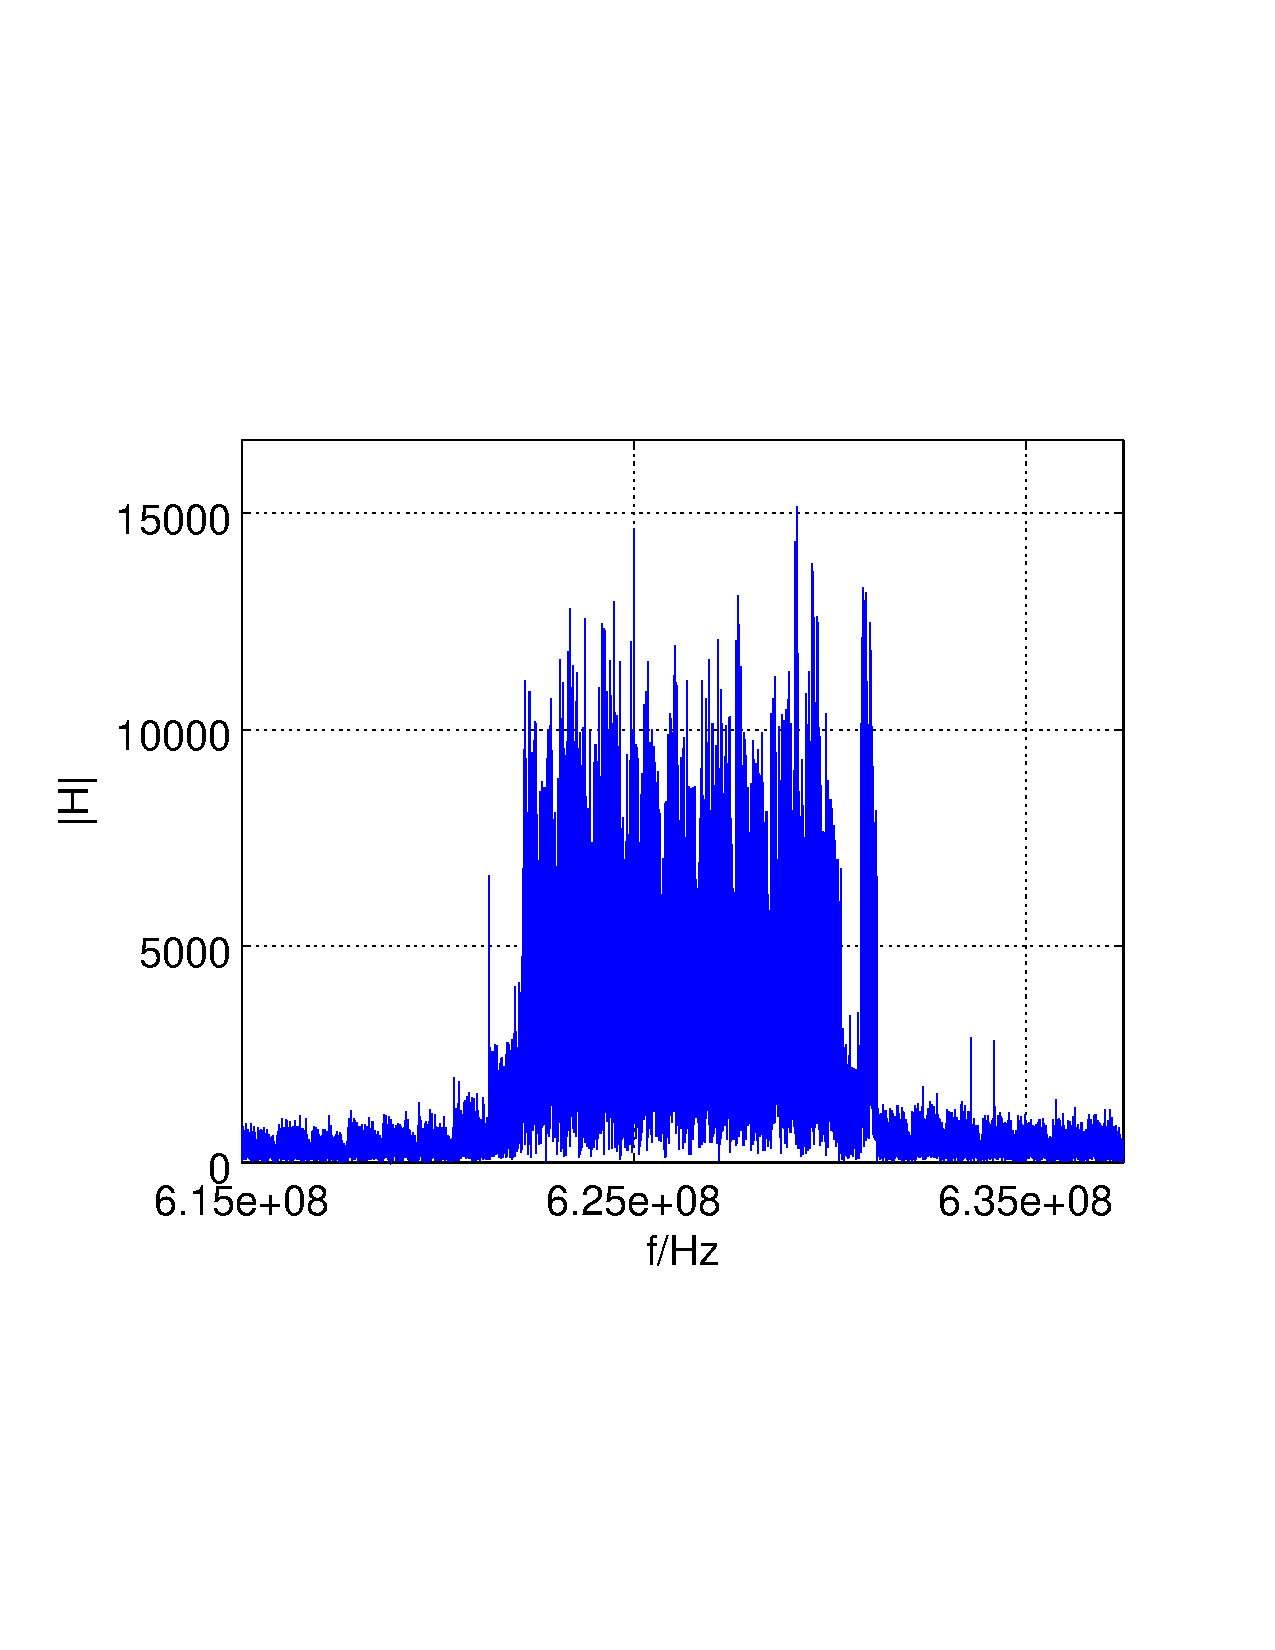
\includegraphics[width=\columnwidth]{./fig/626mhz_raw}
	\end{minipage}
	\hfill
	\begin{minipage}{0.49\columnwidth}
	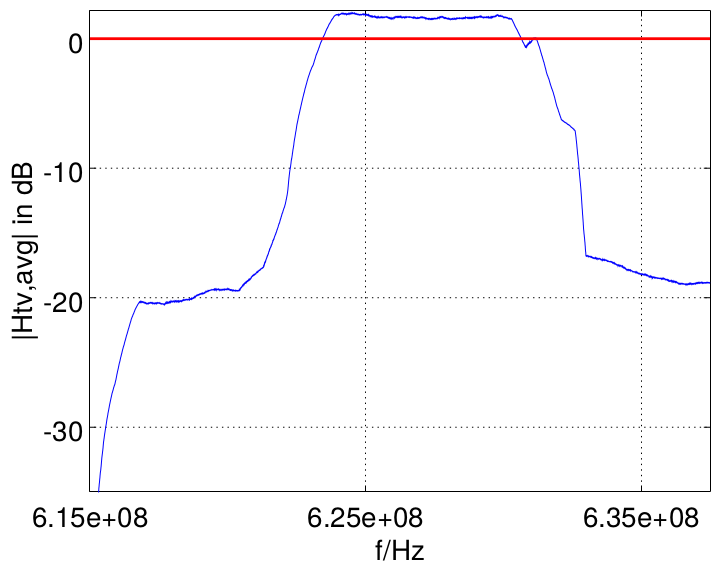
\includegraphics[width=\columnwidth]{./fig/626mhz_filtered}
	\end{minipage}
	\caption{Spectrum of the TV signal. Right: Raw spectrum of the TV signal with \ensuremath{f_{\text{center}}=\text{626 Mhz}}. Left: Smoothed spectrum, normalized to maximum average measured in decibel with average shown as red line.}
	\label{fig:tv_record} 
\end{figure}

We have used the \textit{RTL-SDR} to observe the space variations of the
signal strength. \textit{Octave} scripts have been written to aid in
this purpose. These scripts are available online under
\url{https://github.com/s3xm3x/RTLSDRspecAn}. The scripts perform a
frequency sweep through the desired band. The obtained samples are then
transferred from the time domain to the frequency domain using a fast
fourier transformation (FFT). 

Because the RTL-SDR has a maximum (stable) sampling rate of 2.4 MSPs, we
are limited to a maximum simultaneous acquisition band of 1.2 MHz. We
are keep a safety margin to the maximum capabilities and sample the
desired frequency band at 900 kHz intervals and stitch these bands
together to form the overall frequency sweep. This approach is valid
only because we are not interested in real-time data.  With this
approach we are able to scan a 20 MHz band in roughly two minutes.

During the scanning process the gain is set to 40.2 dB. To get the
signal strength we simply take the average over a 10 MHz band around the
center frequency of the desired TV signal. This approach can be
justified by the fact, that DVB-T is specified up to 10 MHz bandwidth.
And the local TV signal provider is to its own statements using DVB-T 2.
The signal \ensuremath{|H|} is calculated as follows.  
\begin{equation}
	|H| = \Biggl| \sum_{n=0}^N FFT\biggl( \Re\{ s_{\text{band,n}}(t) \} \biggr) \Biggr|
\end{equation}     
where \ensuremath{N} is the total number of intervals accumulated over
the entire frequency sweep. The FFT
is only carried out over the real values, which are received from the
\textit{RTL-SDR}. \ensuremath{s_{\text{band,n}}(t)} is the signal in the
time domain of one interval (one subband). There are as many samples taken in one band as
needed for an FFT of size 2048. To finally get \ensuremath{|H_{tv,avg}|} one has to normalize everything and calculate the power. Before doing that a simple smoothing algorithm (FIR) is applied on \ensuremath{|H|}.
\begin{equation}
	|H_{tv,avg}| = 20 \cdot log (|H|) - 20 \cdot log(|H_0|)
\end{equation}   
where \ensuremath{|H_0|} is a normalization value measured at a certain
point in space. 
\begin{figure}[h]
	\centering
	\begin{minipage}{0.49\columnwidth}
	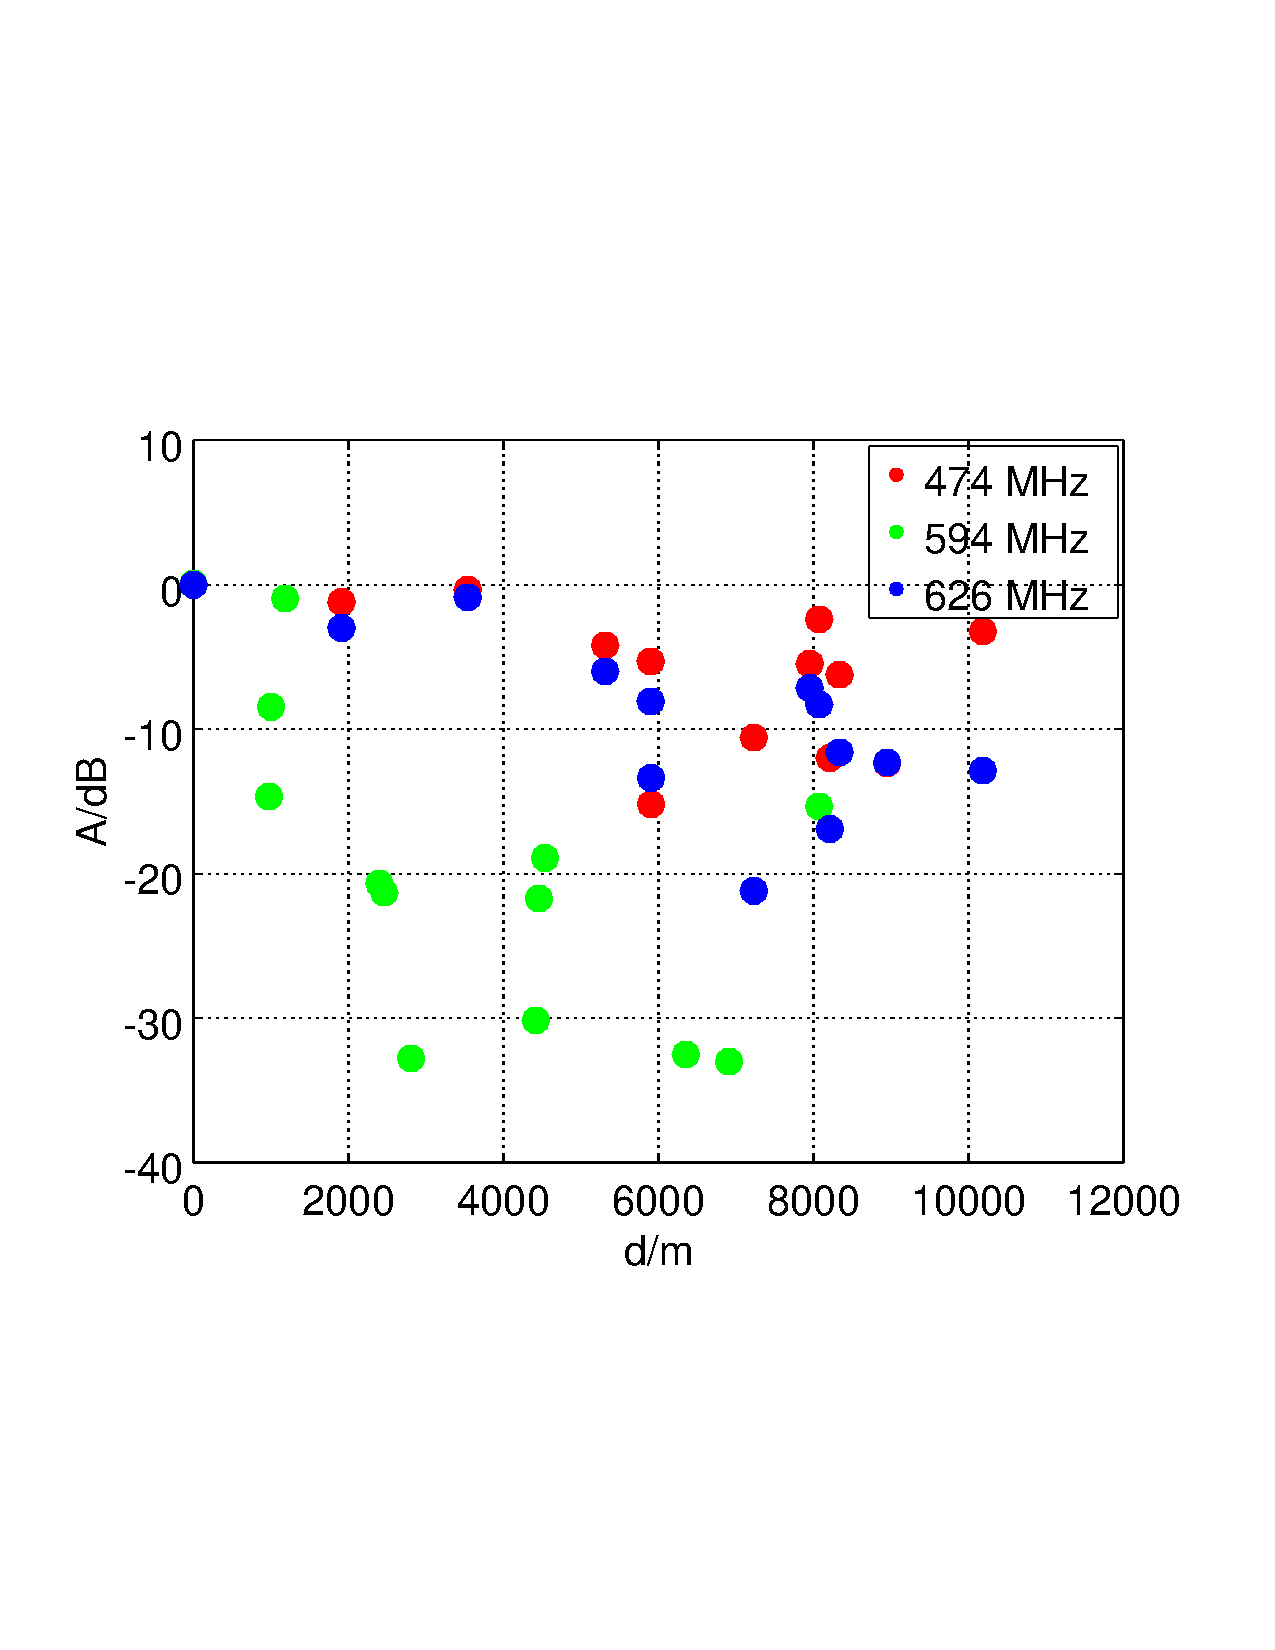
\includegraphics[width=\columnwidth]{./fig/haversine}
	\end{minipage}
	\hfill
	\begin{minipage}{0.49\columnwidth}
	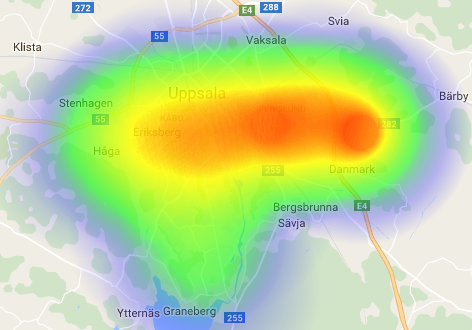
\includegraphics[width=\columnwidth]{./fig/heatmap_626mhz}
	\end{minipage}
	\caption{Left: Signal strength fading against distance relative
to the spot where the maximum signal strength has been captured (TV
towers). 474 MHz and 626 MHz belong to a tower in Uppsala, Vedyxa and
594 MHz belongs to a tower in Uppsala, Rickomberga. Distances have been
calculated with the Haversine formula. Right: Heatmap of the 626 MHz TV
signal in Uppsala.}
 
\label{fig:haversine}
\end{figure}

\subsection{Communication Performance}
We tested the communication with different data rates from 1 bit/s up to
1 kbit/s. As one can see in figure \ref{fig:transmission} the signal
strength is quite low after backscattering. So the problem appears, that
not all bits of the A/D converter are used. Hence a lot of quantization
noise is introduced. In other words more gain is needed. The
transmission shown in figure \ref{fig:transmission} was carried out with
the maximum gain of 50 dB, which is available with the in
\ref{sub:rtl2832} decribed tuner. So we got to the limits of the
\textit{RTL-SDR} at that point. We were able to achieve a range indoors
with 1 bit/s of a couple of meteres, but when we use a higher bitrate we
can only communicate over a range of a couple of decimeter and still
have a bit error ratio of approximately 40 \%. The communiction
experiment was also carried out outside closer to the tower. We could
not figure out any improvements going closer to the tower.  
\section{Discussion}
We are aware of the fact, that our communication system has to be improved until it is able to be used in allday technology. These are aspects, where fine tuning is necessary to enhance the performance:
\begin{itemize}
	\item Antennas: Different backscattering antennas have to be
tried out to find the one with the best results. The question is mainly
to which frequency the antenna has to be tuned (e.g. to the center of
the TV signal or more to the edge of it). Moreover the standard
\textit{RTL-SDR} antenna including the coaxial cable are of quite low
quality. The antenna is e.g. too short. 
	\item Receiver: Some fine tuning can be made when it comes to the filter coefficients of the different filters.
	\item Frame: The frame structure can be optimized to be able to correct errors (e.g. Hamming code).  
\end{itemize}   
To come to a conclusion one can say, that we were able
\begin{itemize}
	\item to show, that spectrum scanning over a huge band with sweeping is possible using the \textit{RTL-SDR}.
	\item to provide a heat map of TV signals in a mid-sized swedish city as well as the tools to create it.
	\item to show for the first time, that backscatter communication is possible with the \textit{RTL-SDR}.
\end{itemize}


% conference papers do not normally have an appendix


% use section* for acknowledgment
%\section*{Acknowledgment}


%The authors would like to thank...





% trigger a \newpage just before the given reference
% number - used to balance the columns on the last page
% adjust value as needed - may need to be readjusted if
% the document is modified later
%\IEEEtriggeratref{8}
% The "triggered" command can be changed if desired:
%\IEEEtriggercmd{\enlargethispage{-5in}}

% references section
\bibliographystyle{IEEEtran}
\bibliography{paper}

\end{document}



